\newpage
\section{Calcolo proposizionale}
\subsection{Dimostrazione di teoremi}
Fin qui abbiamo visto come determinare la conseguenza logica tramite il model checking,
enumerare i modelli e mostrare che la formula deve valere in tutti. La conseguenza logica puo’ essere ottenuta anche tramite la
dimostrazione di teoremi:
\begin{itemize}
    \item applicando regole di inferenza direttamente alle formule della KB
    \item costruire una dimostrazione della formula desiderata senza consultare i modelli
\end{itemize}
Per quest'utlimo caso abbiamo tre fondamentali concetti relativi alla conseguenza logica: equivalenza logica, validià, soddisfacibilità

\subsubsection{Equivalenza logica}
Due formule $\alpha$ e $\beta$ sono \textbf{equivalenti} se sono vere nello stesso insieme di modelli.
$$\alpha \equiv \beta \Leftrightarrow \alpha \models \beta \text{ e } \beta \models \alpha$$
\begin{example}
    $A \land B \equiv B \land A \hspace{10pt} \lnot(A \land B) \equiv \lnot A \lor \lnot B \hspace{10pt} (A \land (A \lor B)) \equiv A$ 
\end{example}
\begin{figure}[h!]
    \centering
    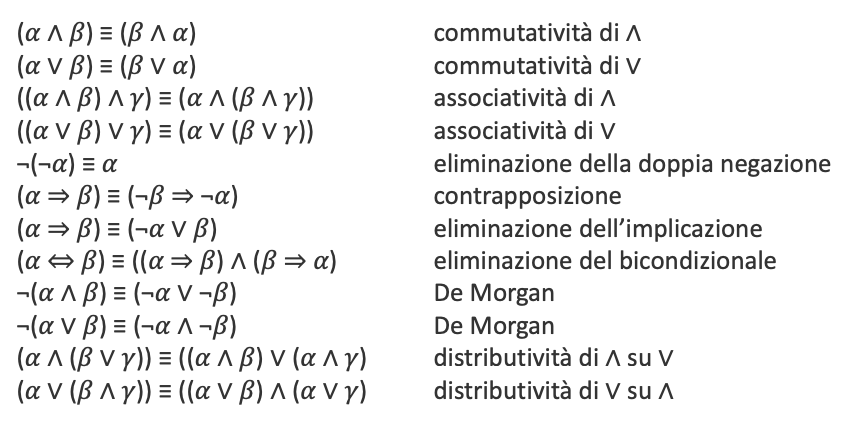
\includegraphics[width=0.65\textwidth]{images/equiv-lofiche.png}
\end{figure}

\subsubsection{Validità}
Una formula $\alpha$ \textbf{valida} sse è vera in tutte le interpretazioni.
\begin{example}
    $A \lor \lnot A$
\end{example}
\hspace{-15pt}Le formule valide sono anche dette \textbf{tautologie}, sono formule necessariamente vere.
\begin{theorem}[Teorema di deduzione]
    Date due formule $\alpha$ e $\beta$ 
    $$\alpha \models \beta \Leftrightarrow (\alpha \Rightarrow \beta) \text{ è valida}$$
\end{theorem}

\subsubsection{Soddisfacibilità}
Una formula $\alpha$ è \textbf{soddisfacibile} sse esiste una interpretazione in cui $\alpha$ è vera (ovvero se esiste un modello di $\alpha$).
\textbf{SAT}: determinare la soddisfacibilità di formule della logica proposizionale.\\\\
Validità e soddisfacibilità sono strettamente connesse:
\begin{itemize}
    \item $\alpha$ è valida sse $\lnot\alpha$ è insoddisfacibile
    \item $\alpha$ è soddisfacibile sse $\lnot\alpha$ non è valida
\end{itemize}

\subsubsection{Dimostrazione per assurdo}
Teorema di deduzione: $\alpha \models \beta$ se e solo se $(\alpha \Rightarrow \beta)$ \textbf{è valida}.\\
$\alpha \models \beta$ se e solo se $\lnot(\alpha \Rightarrow \beta)$ \textbf{è insoddisfacibile}.
Poi applico delle equivalenze logiche:
$$(\alpha \Rightarrow \beta) \equiv (\lnot\alpha \lor \beta) \text{ [eliminazione dell'implicitazione]}$$
$$\lnot(\alpha \Rightarrow \beta) \equiv \lnot (\lnot \alpha \lor \beta) \equiv (\alpha \land \lnot \beta) \text{ [De Morgan]}$$
Da questo consegue che:
$$\alpha \models \beta \Leftrightarrow (\alpha \land \lnot \beta) \text{ è insoddisfacibile}$$
Dimostrazione per refutazione o per contraddizione, si assume che $\beta$ sia falsa e si dimostra che questo porta a una contraddizione
con gli assiomi $\alpha$

\subsubsection{Inferenza per PROP}
\begin{itemize}
    \item \textbf{Model checking}: una forma di inferenza che fa riferimento alla definizione di
    conseguenza logica (si enumerano i possibili modelli), Tecnica delle tabelle di verità (TV)
    \item Algoritmi per la \textbf{soddisfacibilità (SAT)}: $KB \models \alpha \Leftrightarrow (KB \lor \lnot \alpha)$ è insoddisfacibile (\textbf{Teorema di refutazione})
    \begin{itemize}
        \item dimostrare $\alpha$ partendo da KB verificando che ($KB \land \lnot \alpha$) non è mai vero (dimostrazione per assurdo)
        \item si parte da $\lnot \alpha$ e si dimostra che questo porta a una contraddizione con gli assiomi in KB (che sono noti).
    \end{itemize}  
    La conseguenza logica può essere ricondotta a un problema SAT
\end{itemize}

